%%%% main.tex (MIT Sloan SSAC27 submission)
%%%% Carry-Over Lottery Allocation:
%%%%   configuration space + manipulation bound + historical backtest

\documentclass[11pt,letterpaper]{article}

\usepackage[utf8]{inputenc}
\usepackage[T1]{fontenc}
\usepackage{times}
\usepackage[margin=1in]{geometry}
\usepackage{url}
\usepackage[hidelinks]{hyperref}
\usepackage[small]{caption}
\usepackage{graphicx}
\usepackage{amsmath}
\usepackage{amssymb}
\usepackage{amsthm}
\usepackage{booktabs}
\usepackage{array}
\usepackage{multirow}
\usepackage{algorithm}
\usepackage{algorithmic}
\usepackage[numbers]{natbib}

\urlstyle{same}

% Theorem environments
\newtheorem{theorem}{Theorem}
\newtheorem{lemma}[theorem]{Lemma}
\newtheorem{proposition}[theorem]{Proposition}
\newtheorem{corollary}[theorem]{Corollary}
\newtheorem{definition}{Definition}
\newtheorem{remark}{Remark}

% Macros
\newcommand{\cola}{\textup{\textsc{Cola}}}
\newcommand{\Max}{\textup{\textsc{Max}}}
\newcommand{\E}{\mathbb{E}}
\newcommand{\Prob}{\mathbb{P}}

\title{The Carry-Over Lottery Allocation Family:\\Bounds, Backtests, and a Configuration Space for NBA Draft Reform}

\author{
  Timothy Highley\thanks{La Salle University. \texttt{highley@lasalle.edu}}
  \and
  Kaushik Rajan\thanks{Independent researcher. \texttt{kaushi@alumni.ncsu.edu}}
}

\date{\today}

\begin{document}

\maketitle

\begin{abstract}
The annual NBA draft is a constrained fair-allocation problem: 30 indivisible draft picks are assigned to 30 teams that take turns making selections. The top picks are allocated through a lottery for the 14 non-playoff teams. The lottery has a documented manipulation incentive (``tanking''): a team eliminated from playoff contention can improve its expected draft position (DP) by losing additional games. \citet{munro2020notanking} prove an impossibility result, showing that no mechanism based on end-of-season records alone can simultaneously reward poor performance and eliminate this incentive. Carry-Over Lottery Allocation (\cola{}) sidesteps the impossibility by replacing single-season records with a multi-year playoff history as the basis for DP \citep{highley2026cola}. We formalize the \cola{} mechanism family as a configuration space parameterized by seven design dials (eligibility, increment, diminishment, lottery weighting, cap, carry-over scope, tiebreak). Each variant proposed in \citet{highley2026cola} and the Substack series is a point in this space, and the NBA's 2026 ``3-2-1'' proposal sits at a degenerate corner. We instantiate the framework in an empirical testbed against the ZenGM Basketball-GM engine (Section~\ref{sec:empirical}), grid-searching 48 configurations across the dial space (eligibility $\times$ cap $\times$ carry-over scope) under 50 replicates per configuration of 30 simulated seasons. Under universal-dominance comparison on three league-relevant objectives (maximum years between conference-finals appearances, manipulation gain, rank-1-to-5 lottery spread), Capped \cola{} at $\Max = 150$ is the only named variant on the Pareto frontier; Status quo, Classic, Simple, and 3-2-1 are all dominated. Three of the five Pareto-optimal configurations adopt reset-on-championship carry-over scope and three use the 22-team broad eligibility pool. As supporting analytical properties of specific dial configurations, we derive a closed-form $\sim 4\%$ upper bound on the worst-case probability gain from pool manipulation in the Classic configuration (Theorem~\ref{thm:bound}) and a per-series tanking bound for the Capped configuration (Lemma~\ref{lem:capped-bound}). A corollary of the latter shows that the cap value $C$ cancels out of the Capped configuration's manipulation-gain bound, which depends only on the eligibility pool size: $\Delta p_{\text{capped}} \leq 0.3 / |E|$ in the play-in worst case. The empirical sweep confirms the cancellation across $C \in \{100, 150, 200\}$ within each eligibility setting. A 26-season historical backtest (1999--2025) reproduces the Philadelphia ``Process'' as a second-tier validation alongside the headline Pareto result.
\end{abstract}

\section{Introduction}

In the 2025-26 NBA season, multiple teams were publicly accused of tanking in anticipation of a strong draft class. The accusations did not name a small minority: by some counts, roughly a third of the league's 30 teams were openly losing games at season's end to improve their lottery odds. In response, the league introduced a number of potential draft reform ideas, including the ``3-2-1 lottery.'' \citep{highley2026solvable5}. The proposal includes a three-year re-evaluation provision, which means the design discussion is expected to reopen in 2029.

The annual NBA draft is a constrained fair-allocation problem. Thirty indivisible items (draft picks) are assigned to 30 agents (teams) in priority order. Picks 15--30 are assigned by reverse regular-season record. Picks 1--14 are subject to a lottery confined to the 14 non-playoff teams, with weighted odds tilted toward teams with worse records. (In the current system, the bottom three teams are weighted equally and the rest declining). Throughout the years, the NBA has adjusted odds while facing the same question: how to assign indivisible items to agents while (a) preferentially rewarding the weakest agents, (b) eliminating the incentive to under-perform, and (c) producing a mechanism transparent enough that fans, owners, and players can reason about it.

\citet{munro2020notanking} give a formal treatment of the central tension and prove an impossibility. They define a \emph{No-Tanking Condition} (NTC): no team can improve its expected outcome by losing. Any mechanism mapping end-of-season records to draft probabilities, while giving worse-record teams strictly better odds, must violate NTC. Only a uniform lottery (equal odds for all non-playoff teams) satisfies NTC, abandoning differential reward. The 2026 ``3-2-1 lottery'' proposal takes precisely this route, with adjustments for the play-in tournament and reduced odds for the three teams at the bottom of the standings\citep{highley2026solvable5}.

Carry-Over Lottery Allocation (\cola{}) sidesteps the impossibility by replacing single-season records with multi-year playoff history as the basis for draft priority \citep{highley2026cola}. Each non-playoff team accumulates draft priority over consecutive seasons; success in the playoffs or the draft itself diminishes a team's draft priority. The single-season manipulation channel that drives the Munro-Banchio counterexample becomes ineffective: no single-season choice materially shifts the multi-year ticket pool. \cola{} is a family of mechanisms rather than a single design; the original paper develops one concrete instance (\emph{Classic \cola{}}), and subsequent work introduces variants that occupy different points in the design space.

\paragraph{Contributions:}
\begin{itemize}
    \item \textbf{(Section~\ref{sec:family}) A seven-dial configuration space for the \cola{} family.} We formalize the \cola{} mechanism family as a 7-tuple $(E, \Delta, \rho, W, C, S, T)$ specifying eligibility, increment, diminishment, lottery weighting, cap, carry-over scope, and tiebreak (Definition~\ref{def:configuration}). Each variant in the family (Simple, Simple Lottery, Classic, Countdown, Capped) is a point in this space, and the NBA's 2026 ``3-2-1'' proposal sits at a degenerate corner of the same space. Each dial maps to a downstream league-relevant property (incentive compatibility, manipulation gain, per-series cost, transparency), converting variant comparison from a prose comparison to a tuple comparison.
    \item \textbf{(Section~\ref{sec:empirical}) A Basketball-GM empirical testbed and Pareto frontier in the dial space.} We instantiate the configuration space against the ZenGM Basketball-GM engine and compute the Pareto frontier in a 48-configuration grid over eligibility $\times$ cap $\times$ carry-over scope, under 50 replicates per configuration of 30 simulated seasons. Three league-relevant objectives drive the dominance comparison: maximum years between conference-finals appearances (lower is better), manipulation gain (lower is better), and rank-1-to-5 lottery spread (higher is better). Under universal-dominance comparison, Capped \cola{} at $\Max = 150$ is the only named variant on the Pareto frontier; Status quo, Classic, Simple, and 3-2-1 are all dominated.
    \item \textbf{(Sections~\ref{sec:bound} and~\ref{sec:empirical}) Supporting analytical properties: a unified manipulation-gain bound and a cap-cancels-out corollary, with empirical confirmation.} We derive a closed-form upper bound of approximately $4\%$ on the maximum probability gain from pool manipulation under reasonable index distributions (Theorem~\ref{thm:bound}), and a per-series tanking bound for the Capped configuration (Lemma~\ref{lem:capped-bound}). Corollary~\ref{cor:cap-cancels} shows that the cap value $C$ cancels out of the Capped configuration's manipulation-gain bound, which depends only on the eligibility pool size $|E|$. The empirical sweep (Section~\ref{sec:sweep-cap-cancels}) confirms the cancellation: all capped configurations at $|E| = 22$ realize manipulation gain $1.364\%$, all at $|E| = 14$ realize $2.143\%$, and all 16-tiered capped configurations realize $1.875\%$, invariant across $C \in \{100, 150, 200\}$. The 26-season historical backtest (1999--2025) with the 2013--2017 Philadelphia ``Process'' case study is a second-tier validation of the framework alongside the headline Pareto result.
\end{itemize}

\section{Background and Related Work}
\label{sec:background}

\subsection{Effort Manipulation: The Munro-Banchio Impossibility}

\citet{munro2020notanking} establish that any mechanism mapping end-of-season records to draft probabilities, while giving the worst team strictly better odds, must violate NTC. The proof constructs a minimal counterexample: two eliminated teams with identical records and a final game between them. The loser finishes with a worse record and therefore receives better draft odds; both teams prefer to lose. Only the uniform lottery satisfies NTC, but uniform odds abandon the goal of differentially rewarding the weakest teams.

The authors propose \emph{T-IC} (Truncated Incentive Compatibility) as an alternative. T-IC tracks each team's conditional probability of finishing last and freezes allocations at the moment IC would first be violated. The mechanism is optimal in theory but has three practical issues. First, it is opaque to fans. Second, calculating when IC would first be violated requires precise team-level valuations of playoff-versus-draft trade-offs that the league does not have access to. Third, the truncation timing assumes teams have an incentive to win at the start of the season, but some teams have an incentive to tank from the first game.

\subsection{Preference Manipulation and Axiomatic Limits}
\label{sec:fairdiv}

A second impossibility addresses preference misreporting (a team claiming to want a player it does not actually want, to manipulate the allocation order): \citet{coreno2022axiomatic} prove that no draft rule simultaneously satisfies Respect for Priority \citep{svensson1994allocation}, Envy-Free up to One Object \citep{lipton2004approximately,budish2011combinatorial}, and Strategy-Proofness. The result is single-period and applies to one-shot allocations of indivisible items. Whether the axioms lift to the multi-year priority structure of \cola{} is open work outside the scope of this paper; we note the parallel impossibility here as a complement to the Munro-Banchio effort-manipulation channel that motivates the bound in Section~\ref{sec:bound}.

\subsection{Prior Reform Proposals}
\label{sec:priors}

Three reform proposals are the immediate context for \cola{}. The \emph{uniform lottery} (equal odds for all non-playoff teams) is the only mechanism satisfying Munro-Banchio's NTC; it abandons differential reward and the league has not adopted it. The \emph{wheel} (a pre-committed rotation of draft positions across teams, attributed informally to Mike Zarren) eliminates tanking by decoupling record from draft odds, at the cost of removing the rebuilding mechanism for weak teams. The 2026 \emph{3-2-1 lottery} \citep{highley2026threetwoone} expands the lottery to 16 teams across four tiers ($2{:}3{:}2{:}1$ balls per tier from the worst-record tier down) and includes the play-in losers; structurally it is a uniform lottery with adjustments for the play-in and a reduction for the bottom three teams, accepting the Munro-Banchio tradeoff. \cola{} takes a different route: instead of flattening single-season odds, it shifts the priority basis from single-season records to multi-year playoff history, an axis neither Munro-Banchio nor 3-2-1 considers.

\section{The COLA Mechanism Family: A Configuration Space}
\label{sec:family}

\cola{} is a family of mechanisms parameterized by seven design dials. Each NBA lottery reform proposal under recent discussion (the status quo weighted lottery, the 2026 ``3-2-1'' proposal, and each \cola{} variant proposed in \citet{highley2026cola} and the Substack series) corresponds to a specific choice of values for those seven dials. The framework is the league's design lever: a policymaker who wants to move a downstream property (anti-tanking strength, weak-team rebuild horizon, broadcast complexity, multi-year predictability) is moving one or more dials. We organize the section in four parts: the lottery index as the family's unified state variable (Section~\ref{sec:cola-index}), the seven dials that complete the configuration (Section~\ref{sec:seven-dials}), the variant map populating the dials for each proposal under consideration (Section~\ref{sec:variant-map}), and the mapping from dials to league-relevant properties (Section~\ref{sec:dial-properties}). Incentive compatibility for the family is closed by five assumptions \citep{highley2026cola}, summarized in Section~\ref{sec:cola-ic}.

\subsection{Lottery Index}
\label{sec:cola-index}

Every \cola{} variant maintains a per-team, integer-valued state across seasons and uses that state to determine draft priority (DP) in the current season. We refer to this state as the \emph{lottery index} and write $L_i^{(t)}$ for team $i$ at the end of season $t$. Depending on the variant, $L_i^{(t)}$ may track drought length (consecutive seasons without a playoff series win or top-3 pick) or a stockpile of lottery tickets; both are manifestations of the same index.

\begin{definition}[Lottery Index]
\label{def:index}
For each team $i$ and season $t$, the lottery index $L_i^{(t)} \in \mathbb{Z}_{\geq 0}$ is determined by an initial value $L_i^{(0)}$, a per-season \emph{increment} $\Delta_i^{(t)}$ (variant-specific, depending on team performance and eligibility), and a per-season \emph{diminishment} $\rho_i^{(t)} \in [0, 1]$ that scales the index down based on playoff and draft outcomes:
\begin{equation}
\label{eq:index-update}
L_i^{(t+1)} = \left(L_i^{(t)} + \Delta_i^{(t)}\right) \cdot \left(1 - \rho_i^{(t)}\right).
\end{equation}
The \emph{pool} in season $t$ is $P^{(t)} = \sum_{i \in E^{(t)}} L_i^{(t)}$, where $E^{(t)} \subseteq \{1, \ldots, 30\}$ is the set of teams eligible for the lottery in that season.
\end{definition}

The three components of the update (the eligibility set $E^{(t)}$, the increment $\Delta_i^{(t)}$, and the diminishment $\rho_i^{(t)}$) are three of the seven dials that distinguish the variants. For a non-playoff team, the increment is positive (the team accumulates priority); for a team that wins a playoff series or a top draft pick, the diminishment is positive (the team consumes some or all of its accumulated priority). Section~\ref{sec:seven-dials} formalizes these three components together with four additional dials that complete the parameterization; Section~\ref{sec:variant-map} maps each variant onto its 7-tuple in the resulting configuration space.

\subsection{Seven Dials}
\label{sec:seven-dials}

Definition~\ref{def:index} identifies three dials that determine a variant's dynamics: the eligibility set $E^{(t)}$, the increment $\Delta_i^{(t)}$, and the diminishment $\rho_i^{(t)}$. Four additional dials, implicit in the prose definitions of the original paper \citep{highley2026cola} and the Substack series but not yet formalized as design degrees of freedom, complete the configuration: how draft positions are assigned given the index vector, whether the index is bounded above, how long the index persists across seasons, and how identical indices are resolved. We promote these to first-class components of a unified configuration.

\begin{definition}[\cola{} Configuration]
\label{def:configuration}
A \cola{} \emph{configuration} is a 7-tuple $(E, \Delta, \rho, W, C, S, T)$ specifying:
\begin{enumerate}
    \item \textbf{Eligibility} $E^{(t)} \subseteq \{1, \ldots, 30\}$: a season-$t$ predicate selecting the teams that participate in the lottery (per Definition~\ref{def:index}).
    \item \textbf{Increment} $\Delta_i^{(t)} \in \mathbb{Z}_{\geq 0}$: a non-negative integer added to the index of each eligible team, determined by season-$t$ state (per Definition~\ref{def:index}).
    \item \textbf{Diminishment} $\rho_i^{(t)} \in [0, 1]$: the fraction of the index removed after team $i$'s playoff or draft outcome (per Definition~\ref{def:index}).
    \item \textbf{Lottery weighting} $W$: a rule mapping the index vector $L^{(t)}|_{E^{(t)}}$ to a distribution over assignments of teams to draft positions $\{1, 2, \ldots, |E^{(t)}|\}$. The rule may be deterministic (e.g., assign by index rank) or random (e.g., draw pick 1 with probability $L_i / P$, then draw pick 2 from the remainder).
    \item \textbf{Cap} $C \in \mathbb{Z}_{>0} \cup \{\infty\}$: an upper bound on $L_i^{(t)}$, enforced as $L_i^{(t)} \leftarrow \min(L_i^{(t)}, C)$ after each increment. $C = \infty$ denotes no explicit cap.
    \item \textbf{Carry-over scope} $S$: the temporal persistence rule, one of \emph{single-season} (recompute $L_i^{(t)}$ from season-$t$ state alone, no cross-season memory), \emph{unbounded multi-year} (accumulate without limit), \emph{bounded multi-year} (accumulate up to $C$), or \emph{reset-on-event} (clear the index when a specified event occurs).
    \item \textbf{Tiebreak} $T$: a total ordering on $E^{(t)}$ that resolves cases where $L_i^{(t)} = L_j^{(t)}$ for two or more eligible teams.
\end{enumerate}
A \cola{} \emph{variant} is a specification of all seven dials.
\end{definition}

Definition~\ref{def:index} expresses the dynamics of $L^{(t)}$ in terms of dials 1--3; dials 4--7 govern how those dynamics translate into draft positions ($W$), constrain the index's range ($C$) and temporal scope ($S$), and resolve ties ($T$). The four additional dials are not novel mechanisms: each variant in \citet{highley2026cola} and the Substack series specifies a choice for each of them. Formalizing the four implicit choices as typed dials enables two operations: cross-variant comparison via a single configuration object, and dial-by-dial analysis of how each value affects each downstream property. Section~\ref{sec:variant-map} populates the configuration for each variant. Section~\ref{sec:dial-properties} maps the dials to the league-relevant properties that drive the adoption decision.

\subsection{Variant Map}
\label{sec:variant-map}

Table~\ref{tab:variant-map} populates each of the seven dials for the six variants under consideration: the five \cola{} variants and the NBA's 2026 ``3-2-1'' proposal, included as a degenerate configuration (Section~\ref{sec:cola-tank321}). Each row is a dial; each column is a variant. Cell values follow the verbatim specifications in \citet{highley2026cola}, the Substack series \citep{highley2026solvable1,highley2026solvable3,highley2026solvable5}, and Highley's reaction post on the 3-2-1 proposal \citep{highley2026threetwoone}.

\begin{table}[h]
\centering
\footnotesize
\setlength{\tabcolsep}{4pt}
\renewcommand{\arraystretch}{1.25}
\begin{tabular}{@{}c >{\raggedright\arraybackslash}p{0.13\linewidth} >{\raggedright\arraybackslash}p{0.13\linewidth} >{\raggedright\arraybackslash}p{0.13\linewidth} >{\raggedright\arraybackslash}p{0.13\linewidth} >{\raggedright\arraybackslash}p{0.13\linewidth} >{\raggedright\arraybackslash}p{0.13\linewidth}@{}}
\toprule
\textbf{Dial} & \textbf{Simple} & \textbf{Simple Lottery} & \textbf{Classic} & \textbf{Countdown} & \textbf{Capped} & \textbf{3-2-1} \\
\midrule
$E$ & 22 (non-playoff + R1 losers) & 22 (same) & 14 (non-playoff) & 22 (same) & exclusion pool & tiered 16 \\
$\Delta$ & drought $+1$ & drought $+1$ & $\alpha = 1{,}000$ & McCarty $d \cdot w$ & wins $w$ (play-in \& below) & none \\
$\rho$ & reset on series win & reset on series win & 5-step, two channels & reset on advancement & 6-step + 5-step, two channels & none \\
$W$ & deterministic by drought & pre-2019 odds top-14, deterministic rest & $L_i / P$ for picks 1--4, rank for 5--14 & nested-pool MC, tickets $(6,5,4,3,2)$ & $L_i / P$ for picks 1--5, rank for 6+ & tiered balls $(2/3/2/1)$ \\
$C$ & $\infty$ & $\infty$ & $\infty$ & $\infty$ & $\Max = 150$ & n/a \\
$S$ & reset-on-event & reset-on-event & unbounded multi-year & reset-on-event & bounded multi-year & single-season \\
$T$ & most wins & subsumed by $W$ & subsumed by $W$ & subsumed by $W$ & most wins (at cap) & subsumed by $W$ \\
\bottomrule
\end{tabular}
\caption{The seven dials, evaluated for each variant. Dial labels: $E$ eligibility, $\Delta$ increment, $\rho$ diminishment, $W$ lottery weighting, $C$ cap, $S$ carry-over scope, $T$ tiebreak (per Definition~\ref{def:configuration}). The 3-2-1 proposal sits at a degenerate corner: $\Delta$, $\rho$, $C$ are vacuous and $S$ is single-season, leaving only $E$ and $W$ as active dials.}
\label{tab:variant-map}
\end{table}

The variants trade off explainability, anti-tanking strength, and per-series tanking exposure differently. Simple \cola{} \citep{highley2026solvable3} eliminates the lottery in favor of a deterministic ordering on drought, with eligibility extended to first-round losers; Simple Lottery \cola{} \citep{highley2026solvable3} layers the pre-2019 NBA weighted odds on top of Simple's drought ordering. Classic \cola{} is the original variant of \citet{highley2026cola} and the variant our manipulation bound (Section~\ref{sec:bound}) directly analyzes. Countdown \cola{} \citep{highley2026solvable3} uses the McCarty number (drought $\times$ wins) and a nested-pool Monte Carlo draw that guarantees no team falls more than four spots below its priority rank. Capped \cola{} \citep{highley2026solvable5}, introduced in response to the NBA's reported reluctance to adopt a flexible lottery line, adds a wins-based increment, a stockpile cap ($\Max = 150$), and a six-step playoff diminishment schedule; the cap bounds the per-series tanking incentive (Lemma~\ref{lem:capped-bound}). The 2026 NBA ``3-2-1'' proposal \citep{highley2026threetwoone} sits at a degenerate corner: dials $\Delta$, $\rho$, and $C$ are vacuous, $S$ collapses to single-season, and only $E$ (a tiered 16-team pool) and $W$ (a tiered ball allocation) carry the proposal's design. The collapse is the proposal's defining structural feature, not an incidental implementation choice; Section~\ref{sec:cola-tank321} elaborates.

\subsection{Dial-to-Property Mapping}
\label{sec:dial-properties}

The configuration space of Definition~\ref{def:configuration} reduces a variant comparison to a tuple comparison. The comparison is informative only when each dial corresponds to a downstream property of the resulting mechanism. Four properties dominate the league-side adoption discussion: anti-tanking strength (how much within-season manipulation is foreclosed), weak-team rebuild help (how reliably the worst teams accumulate priority), complexity (how legible the mechanism is to fans and media), and predictability (how forecastable a multi-year team trajectory is for general managers and owners). Table~\ref{tab:dial-properties} summarizes the mapping.

\begin{table}[h]
\centering
\footnotesize
\setlength{\tabcolsep}{4pt}
\renewcommand{\arraystretch}{1.25}
\begin{tabular}{@{}c >{\raggedright\arraybackslash}p{0.19\linewidth} >{\raggedright\arraybackslash}p{0.19\linewidth} >{\raggedright\arraybackslash}p{0.19\linewidth} >{\raggedright\arraybackslash}p{0.19\linewidth}@{}}
\toprule
\textbf{Dial} & \textbf{Anti-tanking strength} & \textbf{Weak-team rebuild help} & \textbf{Complexity} & \textbf{Predictability} \\
\midrule
$E$       & Sets the pool $P$ in Theorem~\ref{thm:bound}; narrower pools admit larger gain     & Determines which weak teams accumulate priority    & High if simple count, low if exclusion-rule         & Stable if record-based; less so if exclusion-rule \\
$\Delta$  & Bounds the per-season marginal-decision gain                                       & Flat $\alpha$ rewards uniformly; $w$-based rewards within-season effort & High if flat, lower if formulaic                    & High if record-based                              \\
$\rho$    & Cliff size at each round transition; controls repeat-tanking returns               & Restores priority to teams missing the playoffs again after success & Medium                                              & Medium                                            \\
$W$       & Spread across rank positions; decouples position from index in part                & Tilts allocation toward worst-record teams         & High if deterministic, low if Monte Carlo            & High if deterministic, lower if random            \\
$C$       & Bounds $p_{\max}$ and the per-series cost (Lemma~\ref{lem:capped-bound})           & Low cap compresses the priority signal             & Medium                                              & High once known                                   \\
$S$       & Escapes the \citet{munro2020notanking} impossibility via multi-year scope          & Multi-year scope rewards persistent weakness       & Medium                                              & Lower under multi-year scopes (legal/contracting) \\
$T$       & Edge case for $W$-deterministic variants                                           & n/a                                                & High if simple                                      & High                                              \\
\bottomrule
\end{tabular}
\caption{Dial-to-property mapping. Cell entries describe the form the dial's influence takes; the dials and the variants of Table~\ref{tab:variant-map} together specify how to move from one league-relevant property to another by altering one or more dial values.}
\label{tab:dial-properties}
\end{table}

The mapping logic is direct. Three dials ($E$, $\Delta$, $C$) bound the manipulator's pool share $p_{\max}$ and the size of any pool perturbation: a larger eligible set yields a larger total pool $P$, the increment $\Delta$ bounds the per-team per-season accumulation, and the cap $C$ bounds the index outright. Two dials ($\rho$, $S$) govern multi-year accumulation: the diminishment schedule determines how quickly an index decays after success, and the carry-over scope determines whether accumulation persists at all (the dial whose non-single-season value escapes the \citet{munro2020notanking} impossibility). The remaining two dials ($W$, $T$) translate the index dynamics into draft positions: $W$ determines whether the high-index team gets pick 1 deterministically or in expectation, and $T$ resolves cases where the index is silent. Anti-tanking strength and weak-team rebuild help load on $E, \Delta, \rho, C, S$; complexity loads on $E, W$ (the fan- and media-visible dials) and on $S$ (the league-counsel-visible dial); predictability loads on $\rho, S$ (the multi-year forecasting dials). A league that finds Classic too unbounded can move $C$ to a finite value (the Capped move). A league that finds multi-year scopes administratively heavy can move $S$ to single-season (the 3-2-1 move). The framework's value to a policymaker is that the choice among variants becomes a choice among dial settings, not among monoliths.

\subsection{Incentive Compatibility}
\label{sec:cola-ic}

\citet{highley2026cola} establish incentive compatibility (IC) for Classic \cola{} under five assumptions:
\begin{enumerate}
    \item \textbf{Playoff primacy:} the value to a team of advancing in the playoffs exceeds the value of any plausible draft-pick gain.
    \item \textbf{Playoff advancement:} within the playoffs, advancing further is preferred to losing earlier, controlling for opponent strength.
    \item \textbf{Picks 5--14 negligible at the margin:} no team profits from manipulating its position among those slots through within-season effort.
    \item \textbf{Pool manipulation negligible:} no team can meaningfully shift its expected draft position by manipulating which other teams are in or out of the lottery pool.
    \item \textbf{No traded-pick protections:} pick trades do not interact with diminishment in a way that creates manipulation incentives.
\end{enumerate}
Assumptions (1)--(3) and (5) hold by construction or follow from straightforward arguments. Assumption (4) is supported by \citet{highley2026cola} via a $1{,}000$-season simulation, observing a maximum probability gain of approximately $3\%$. Section~\ref{sec:bound} converts this empirical observation into a closed-form analytic bound for the Classic configuration.

\subsection{The 3-2-1 Proposal as a Degenerate Configuration}
\label{sec:cola-tank321}

The NBA's 2026 reform proposal (``3-2-1''), slated for an owners' vote at the end of May 2026, expands the lottery to sixteen teams across four tiers and assigns ball counts of two, three, two, and one per tier respectively. In the configuration of Definition~\ref{def:configuration}: dials $\Delta$, $\rho$, and $C$ are vacuous; the carry-over scope $S$ is single-season; the eligibility set $E$ is the tiered 16-team pool; the lottery weighting $W$ is the tiered ball allocation; and the tiebreak $T$ is subsumed by the random draw. Three dials ($E$, $W$, $S$) carry the proposal's design. In \citet{highley2026threetwoone}'s framing, the mechanism is ``essentially the uniform lottery but with an adjustment for the play-in and a punishment for the bottom 3 teams.'' By assigning the worst three teams fewer balls than the middle seven, the proposal does not satisfy the premise of the Munro-Banchio counterexample (that worse teams have strictly better odds), and sidesteps the impossibility at the cost of abandoning the rationale for differential odds in the first place. \cola{} takes the opposite route: instead of flattening single-season odds, it shifts the priority basis from single-season records to multi-year playoff history through dial $S$ in modes other than single-season.

\section{Pool Manipulation Bound}
\label{sec:bound}

\subsection{Setup}

Let $P = \sum_{i=1}^{n} L_i$ denote the total lottery pool, where $L_i$ is team $i$'s lottery index and $n$ is the number of lottery-eligible teams. A team's probability of winning the first pick is $p_i = L_i / P$.

The \emph{pool manipulation} channel operates as follows. Team $i$ deliberately loses to a high-index opponent $h$ near the playoff boundary, causing $h$ to make the playoffs. Team $h$ (with index $L_h$) exits the lottery pool and is replaced by a lower-index team $\ell$ (with index $L_\ell < L_h$). The pool shrinks by $\Delta = L_h - L_\ell > 0$.

\begin{proposition}[Manipulation Gain]
\label{prop:gain}
The probability gain for team $i$ from a pool swap of size $\Delta = L_h - L_\ell$ is
$
G_i = L_i \cdot \Delta / [P \cdot (P - \Delta)].
$
\end{proposition}

\begin{proof}
Before manipulation, $p_i = L_i / P$. After the swap, the new pool is $P' = P - \Delta$ and $p_i' = L_i / P'$. The gain is $G_i = p_i' - p_i = L_i \big( 1/(P - \Delta) - 1/P \big) = L_i \cdot \Delta / [P(P - \Delta)]$.
\end{proof}

When $\Delta \ll P$ (typically $\Delta / P \approx 4\%$ in our backtest), the gain factors into two ratios: the manipulator's pool share ($p_i$) and the fractional pool change ($\Delta / P$). Both have structural ceilings, which we exploit below.

\paragraph{Indexing convention.} The bound below uses the expression $L_i = T_i \cdot \alpha$, where $T_i$ is team $i$'s consecutive non-playoff seasons. For Classic \cola{}, this is exact for any team starting from a stockpile reset (a championship or top-5 lottery pick) and is the steady-state attractor under the diminishment schedule. A fully general bound that handles ticket inheritance from earlier playoff series under the full diminishment dynamics is in the broader paper.

\subsection{Conditioned Upper Bound}

\begin{definition}[Structural Anti-Correlation]
\label{def:anticorr}
Let $T_{\max}$ denote the maximum consecutive non-playoff years for any team, and $T_{\text{boundary}}$ the maximum consecutive non-playoff years for a team near the playoff boundary (a team that could plausibly be pushed into the playoffs by a single loss). The index distribution exhibits \emph{structural anti-correlation} when $T_{\text{boundary}} \ll T_{\max}$: teams with the highest indices are far from the playoff boundary and thus cannot be the target of pool manipulation.
\end{definition}

\begin{theorem}[Conditioned Manipulation Bound]
\label{thm:bound}
Under structural anti-correlation with parameters $T_{\max}$, $T_{\text{boundary}}$, and average index multiplier $\bar{k} = \bar{L} / \alpha$, where $\alpha$ is the annual index increment, the maximum manipulation gain satisfies
\begin{equation*}
G_{\max} \leq \frac{T_{\max} \cdot (T_{\text{boundary}} - 1)}{(T_{\max} + n - 1) \cdot n \cdot \bar{k}}.
\end{equation*}
\end{theorem}

\begin{proof}[Proof sketch]
The gain is maximized when $L_i$ is maximized and $\Delta / P$ is maximized. \emph{Bounding $p_{\max}$}: the highest-index team has $L_{\max} = T_{\max} \cdot \alpha$. The minimum pool size occurs when one team has $T_{\max}$ years of accumulation and the remaining $n - 1$ teams each have the minimum $\alpha$: $P_{\min} = (T_{\max} + n - 1) \cdot \alpha$. Thus $p_{\max} \leq T_{\max} / (T_{\max} + n - 1)$. \emph{Bounding $\Delta / P$}: the team being pushed out has at most $T_{\text{boundary}} \cdot \alpha$ tickets, and the team replacing it has at least $\alpha$, so $\Delta_{\max} = (T_{\text{boundary}} - 1) \cdot \alpha$. In steady state, $P \approx n \cdot \bar{k} \cdot \alpha$. Combining via the first-order approximation yields the stated bound.
\end{proof}

\paragraph{Empirical calibration:} We instantiate the bound with $T_{\max} = 10$ (the typical-case ceiling on consecutive non-playoff years across teams in our 26-season backtest), $T_{\text{boundary}} = 5$ (a conservative ceiling on the consecutive non-playoff years a near-boundary team can accumulate before improving enough to clear the boundary), $n = 14$ (the structural count of NBA non-playoff teams), and $\bar{k} = 3.1$ (an average team has roughly three years of carry-over before reset, matching the original paper's observation). These yield
\begin{equation*}
G_{\max} \leq \frac{10 \cdot 4}{23 \cdot 14 \cdot 3.1} \approx 4.0\%,
\end{equation*}
which contains the simulation-observed maximum of $3.0\%$ across $1{,}000$ seasons \citep{highley2026cola}. An independent 200-season Bradley-Terry simulation we ran confirms the bound, with observed maximum gain of $1.70\%$. The 26-season historical dataset contains one outlier: the Sacramento Kings' 16-year drought (2006--07 through 2021--22). Setting $T_{\max} = 16$ to include the outlier loosens the bound to approximately $5.1\%$, still well above the empirical extremes; we report the typical-case bound ($T_{\max} = 10$) as the headline because the next-longest droughts are Minnesota at 13 years and Phoenix and Charlotte at 10 each.

\begin{figure}[t]
\centering
\begin{minipage}{0.48\columnwidth}
\centering
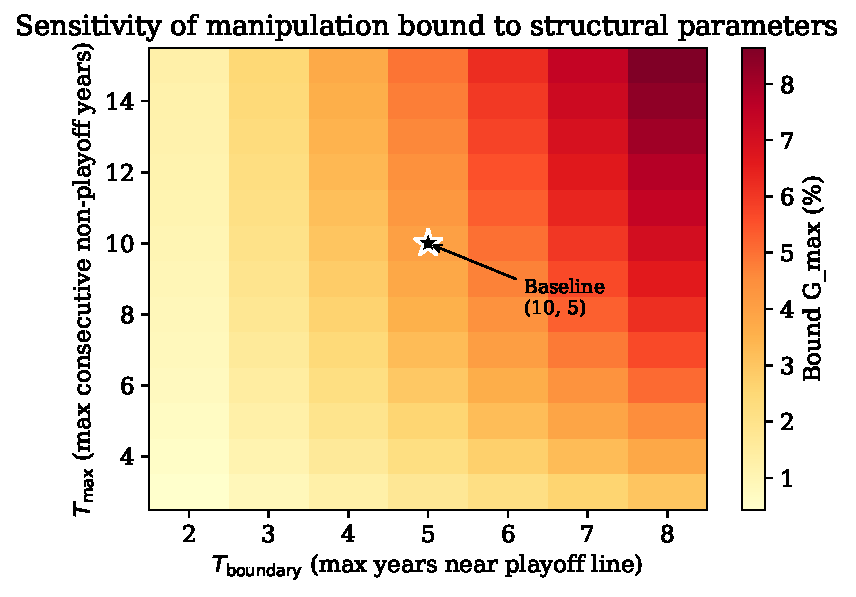
\includegraphics[width=\columnwidth]{figures/bound_sensitivity.pdf}
\caption*{(a) Bound vs.\ $T_{\max}, T_{\text{boundary}}$.}
\end{minipage}\hfill
\begin{minipage}{0.48\columnwidth}
\centering
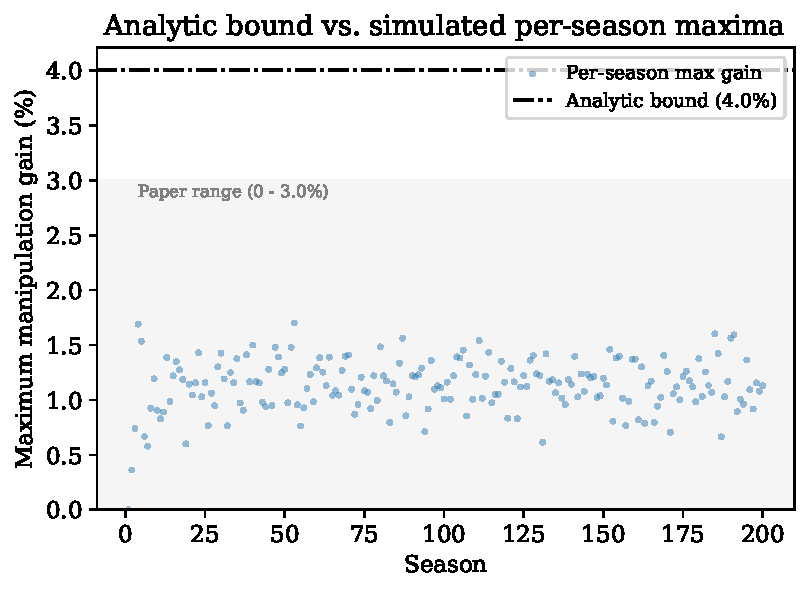
\includegraphics[width=\columnwidth]{figures/bound_vs_sim.pdf}
\caption*{(b) Analytic bound vs.\ simulation.}
\end{minipage}
\caption{Manipulation bound. (a) Sensitivity to the structural-anti-correlation parameters; the bound is most sensitive to $T_{\text{boundary}}$, and stays under $5\%$ for $T_{\text{boundary}} \leq 5$. (b) Analytic bound (red) vs.\ the empirical distribution of manipulation gains across 200 Bradley-Terry-simulated seasons; the bound contains all simulated outcomes with margin.}
\label{fig:bound}
\end{figure}

\subsection{Sensitivity, Coalitions, and the Pick-Value Gap}

The bound's parameter sensitivity (Figure~\ref{fig:bound}a) shows that $T_{\text{boundary}}$ is the dominant lever: even under pessimistic assumptions ($T_{\text{boundary}} = 7$), the bound stays under $7\%$, and under realistic conditions ($T_{\text{boundary}} \leq 5$) it stays under $5\%$. This matters operationally because $T_{\text{boundary}}$ is the empirical quantity most amenable to direct measurement.

For completeness, coalitional manipulation (two or more teams coordinating to shrink the pool) does not amplify individual gains. Joint gain for a coalition $\{A, B\}$ is $(L_A + L_B) \cdot \Delta / [P(P - \Delta)]$. Even at $30\%$ joint pool share, the gain remains $\leq 1.3\%$, and per-member gain cannot exceed the highest-index individual's gain. Coordination costs (detection risk, trust problems, sequential uncertainty) further dampen the channel.

The bound addresses the \emph{probability} term of the manipulation incentive. The \emph{value} term (the pick-value gap $d_k - d_{k+1}$ between adjacent draft positions) has no formal ceiling in the original specification, though it is bounded for any realistic draft class. Closing assumption (4) entirely would also require a separate argument capping $d_k - d_{k+1}$ via the distribution of draft-eligible prospect quality. We leave this to future work.

\subsection{Per-Series Bound for Capped \cola{}}

Capped \cola{} introduces a fourth manipulation channel: tanking through the playoffs themselves (a team within the cap declining to advance, in order to retain its stockpile). The cap converts the playoff-diminishment schedule from a fraction-of-current-stockpile cost (unbounded above when stockpile grows large) to a fraction-of-$\Max$ cost (bounded by construction).

\begin{lemma}[Per-Series Tanking Cost]
\label{lem:capped-bound}
Let $\Max$ be the Capped \cola{} stockpile cap. For any team entering the playoffs with $L_i \leq \Max$, the maximum reduction in $L_i$ attributable to winning (rather than losing) any single playoff series is bounded by:
\begin{equation*}
\Delta L_{\text{series}}^{\max} = \begin{cases}
0.3 \cdot \Max & \text{play-in advancers in round 1,} \\
0.2 \cdot \Max & \text{any other series advancement.}
\end{cases}
\end{equation*}
At $\Max = 150$, the bound is $45$ tickets for the play-in case and $30$ tickets for any subsequent series.
\end{lemma}

\begin{proof}
Reading off Capped \cola{}'s six-step diminishment schedule, the per-series increments in the diminishment fraction $\Delta\rho$ are: play-in advancer round 1 ($\rho_{\text{lose}} = 0.1$, $\rho_{\text{advance}} = 0.4$, $\Delta\rho = 0.3$); standard round 1 ($0.2 \to 0.4$, $\Delta\rho = 0.2$); round 2 to conference finals ($0.4 \to 0.6$); conference finals to NBA finals ($0.6 \to 0.8$); finals to championship ($0.8 \to 1.0$). All non-play-in transitions yield $\Delta\rho = 0.2$. The cost in tickets is $\Delta\rho \cdot L_i^{\text{pre}} \leq \Delta\rho \cdot \Max$, with equality at the cap.
\end{proof}

The bound makes the playoff-tanking incentive transparent at the league level: at $\Max = 150$, no single series win ever costs a team more than $45$ lottery tickets, which is approximately a year and a half of accumulation for a team near the wins-increment ceiling. The cumulative regret for a finals-losing team at the cap is $0.8 \cdot \Max = 120$ tickets, decomposed into per-series increments per Lemma~\ref{lem:capped-bound}.

\begin{corollary}[Cap-Cancels-Out for Capped Configurations]
\label{cor:cap-cancels}
For a Capped \cola{} configuration with eligibility pool $E$ of size $|E|$, cap value $C$, and per-series-cost upper bound $\kappa \cdot C$ (where $\kappa = 0.3$ in the play-in worst case of Lemma~\ref{lem:capped-bound} and $\kappa = 0.2$ for any subsequent series), the worst-case manipulation-gain bound for a single-series pool perturbation is
\begin{equation*}
\Delta p_{\text{capped}} \;\leq\; \frac{\kappa \cdot C}{C \cdot |E|} \;=\; \frac{\kappa}{|E|}.
\end{equation*}
The cap value $C$ drops out. The manipulation-gain bound depends only on $\kappa$ and $|E|$. Section~\ref{sec:sweep-cap-cancels} confirms the cancellation empirically.
\end{corollary}

\begin{proof}
The maximum index a single team can hold under Capped \cola{} is $C$, and the worst-case pool of $|E|$ such teams is $C \cdot |E|$. The maximum single-series perturbation in a team's index from the pool is $\kappa \cdot C$ tickets, by Lemma~\ref{lem:capped-bound}. Substituting into the gain expression $\Delta = (\text{perturbation}) / (\text{pool})$ yields $\kappa \cdot C / (C \cdot |E|) = \kappa / |E|$.
\end{proof}

The corollary clarifies the role the cap plays under Capped \cola{}. The cap controls per-team accumulation speed (how fast a single team builds up advantage relative to the rest of the pool) and the per-series tanking cost (Lemma~\ref{lem:capped-bound}); it does not control pool-wide manipulation resistance. The latter is set by the eligibility pool size $|E|$. A policymaker considering a Capped configuration can therefore tune $C$ on the basis of accumulation-speed and per-series-cost preferences without affecting the manipulation-gain ceiling. At the Capped \cola{} published defaults ($|E| = 22$, $\kappa = 0.3$ play-in or $\kappa = 0.2$ standard), the bound is $\Delta p_{\text{capped}} \leq 0.3 / 22 \approx 1.36\%$ in the play-in worst case and $0.2 / 22 \approx 0.91\%$ for any subsequent series.

\subsection{Three Closures of Assumption (4)}

The pool-manipulation gap (assumption~(4) in Section~\ref{sec:family}) admits at least three closure strategies, each represented in the literature.
\begin{itemize}
\item \textbf{Empirical closure:} \citet{highley2026cola} simulate $1{,}000$ synthetic seasons under Bradley-Terry and observe a maximum gain of $\sim 3\%$. The closure is statistical: the assumption holds in the typical case but admits no parameter-explicit ceiling.
\item \textbf{Behavioral closure:} the companion formal-proof video to \citep{highley2026cola} introduces an additional behavioral assumption $G > $ expected pool-manipulation gain (where $G$ is the value of a single regular-season win), eliminating the channel via preference structure rather than mechanism design.
\item \textbf{Analytic closure (this paper):} Theorem~\ref{thm:bound} provides a closed-form upper bound conditioned on structural properties of the index distribution. The bound is parameter-explicit and admits sensitivity analysis (Figure~\ref{fig:bound}a).
\end{itemize}
The three closures compose: any practical \cola{} deployment can rely on whichever closure best matches the available evidence. Our contribution is the analytic option, which previously did not exist.

\section{Empirical Validation}
\label{sec:empirical}

This section instantiates the configuration space of Section~\ref{sec:family} in an empirical testbed against the ZenGM Basketball-GM engine. Section~\ref{sec:sim-model} discloses the simulation model. Section~\ref{sec:testbed-setup} describes the dial grid, objectives, and Pareto methodology. Section~\ref{sec:pareto-frontier} reports the headline result: under universal-dominance comparison, Capped \cola{} at $\Max = 150$ is the only named variant on the Pareto frontier. Section~\ref{sec:sweep-cap-cancels} confirms the cap-cancels-out result of Corollary~\ref{cor:cap-cancels} empirically. Section~\ref{sec:reset-on-championship} reports the carry-over scope finding: reset-on-championship is the modal winning scope on the frontier. Section~\ref{sec:backtest} carries the 26-season historical backtest as a second-tier validation, and Section~\ref{sec:sensitivity} reports sensitivity at $N = 30$ and $N = 100$.

\subsection{Simulation Model}
\label{sec:sim-model}

The ZenGM Basketball-GM engine implements all five \cola{} variants and the standard NBA lottery; we use it as the canonical reference implementation. ZenGM's browser-coupled \texttt{createLeague()} path does not port cleanly to Node, so the testbed bypasses it and synthesizes regular-season game outcomes: strength-weighted win records and a single-elimination playoff bracket. The real ZenGM lottery code is unchanged: lottery draws use \texttt{draft.genOrder} and per-team \texttt{cola} updates from \texttt{cola.ts}.

Team strength persists across seasons via a Markov model tied to draft outcomes. Let $s_t \in [0, 1]$ denote a team's strength in season $t$, $\rho$ the persistence parameter, $\mu$ the long-run parity mean, $\alpha$ the per-draft impact, $\sigma$ the annual shock standard deviation, $\varepsilon_t \sim \mathcal{N}(0, \sigma^2)$ a Normal shock, and $\pi(p) = \max(0, (16 - p) / 15)$ the value of a draft pick at position $p$ (pick 1 contributes full $\alpha$, pick 15 contributes zero, picks 16 and later contribute zero). The transition is
\begin{equation}
s_{t+1} = \mathrm{clip}\!\big(\rho \, s_t + (1 - \rho) \, \mu + \alpha \, \pi(p_t) + \varepsilon_t, \; 0, \; 1\big),
\label{eq:strength-markov}
\end{equation}
with $\rho = 0.9$, $\mu = 0.5$, $\alpha = 0.15$, and $\sigma = 0.05$. Initial strength is drawn from $\mathrm{Uniform}[0.3, 0.7]$. This preserves the feedback loop the primary objective (worst-franchise gap between conference-finals appearances) is designed to measure: a team's lottery position drives its draft pick, which drives its next-season strength. The model is parametrically calibrated for plausibility, not fit to historical NBA team-strength trajectories; a formal calibration against league rating systems or Basketball Reference strength-of-schedule data is future work.

\subsection{Testbed Setup}
\label{sec:testbed-setup}

The headline sweep grid-searches three dials of Definition~\ref{def:configuration} jointly: eligibility $E$, cap $C$, and carry-over scope $S$. The remaining four dials ($\Delta, \rho, W, T$) are held at the canonical settings each variant inherits from \citet{highley2026cola} and the Substack series. The dial grid is
\begin{itemize}
    \item Eligibility $E \in \{14, 22, \text{16-tiered}\}$: 14-team non-playoff pool (Classic, Status quo); 22-team broad pool including round-1 losers (Simple, Capped); 16-team tiered pool of the 2026 3-2-1 proposal.
    \item Cap $C \in \{\text{uncapped}, 100, 150, 200\}$: uncapped reproduces Classic / Simple; $C = 150$ is the Capped \cola{} default \citep{highley2026solvable5}.
    \item Carry-over scope $S \in \{\text{single-season}, \text{unbounded}, \text{bounded-30yr}, \text{reset-on-championship}\}$: single-season collapses to the 3-2-1 / Status-quo behavior; unbounded reproduces Classic; bounded-30yr is the Capped default; reset-on-championship clears every team's lottery index when the league champion is decided each season.
\end{itemize}
The grid yields $3 \times 4 \times 4 = 48$ configurations. The headline run executes each configuration under $50$ replicates (seeds $1000$ through $1049$, deterministic via overridden \texttt{Math.random}) of $30$ simulated seasons each, for $2{,}400$ \texttt{(config, replicate)} rows.

Each \texttt{(config, replicate)} row reports four objectives. The three dominance dimensions are: (i) the maximum number of years between conference-finals appearances for any franchise (lower is better; the primary parity objective, suggested by Prof.\ Highley); (ii) the analytical manipulation-gain bound $\Delta p$ for the configuration, expressed as a percentage (lower is better; closed-form from $E$ and $C$, no Monte Carlo); (iii) the rank-1-to-5 lottery spread (higher is better; the gap between the worst team's expected pick and the fifth-worst team's expected pick under the lottery). The fourth column is the per-series cost ceiling from Lemma~\ref{lem:capped-bound} (lower is better; not used for dominance because it is N/A for uncapped configurations).

A configuration is Pareto-optimal under \emph{3-objective universal dominance}: no other configuration in the grid is weakly better on all three dimensions and strictly better on at least one. Per-configuration summaries take the median across the $50$ replicates (the median is less sensitive than the mean to extreme-value outliers in max-gap statistics). Section~\ref{sec:sensitivity} reports a stability check at $N = 30$ and $N = 100$ on a subset that pools the headline Pareto-optimal set with the five named variants.

\subsection{Pareto Frontier}
\label{sec:pareto-frontier}

Five of the 48 configurations are Pareto-optimal under 3-objective universal dominance (Table~\ref{tab:pareto-set}). Among the named variants, only Capped \cola{} at $\Max = 150$ (configuration 26) is on the frontier; Status quo (configuration 0), Classic (configuration 1), Simple (configuration 17), and 3-2-1 (configuration 32) are all dominated. Capped \cola{} achieves the joint minimum manipulation gain of $1.364\%$ and the maximum rank-1-to-5 spread of $2.867$ on the frontier, dominating Status quo at every objective. Figure~\ref{fig:pareto-manip} visualizes the dominance picture in the (max-yrs-CF, manipulation-gain) plane.

\begin{table}[t]
\centering
\small
\setlength{\tabcolsep}{4pt}
\begin{tabular}{rrrr@{\hspace{6pt}}rrr@{\hspace{6pt}}l}
\toprule
cid & $E$ & $C$ & $S$ & max-yrs-CF & $\Delta p$ [\%] & rank-spread & named variant \\
\midrule
11 & 14 & 150 & reset-on-championship & 27.0 & 2.143 & 2.433 &  \\
19 & 22 & uncapped & reset-on-championship & 26.0 & 18.182 & 2.650 &  \\
26 & 22 & 150 & bounded-30yr & 28.0 & 1.364 & 2.867 & Capped@150 \\
31 & 22 & 200 & reset-on-championship & 27.5 & 1.364 & 2.667 &  \\
45 & 16-tiered & 200 & unbounded & 27.5 & 1.875 & 2.700 &  \\
\midrule
\multicolumn{8}{c}{\textbf{Named variants under unified units (all dominated except Capped@150)}} \\
\midrule
0 & 14 & uncapped & single-season & 28.5 & 28.571 & 2.767 & Status quo \\
1 & 14 & uncapped & unbounded & 27.5 & 28.571 & 2.367 & Classic \\
17 & 22 & uncapped & unbounded & 29.0 & 18.182 & 2.667 & Simple \\
32 & 16-tiered & uncapped & single-season & 28.0 & 25.000 & 2.567 & 3-2-1 \\
\bottomrule
\end{tabular}
\caption{The five Pareto-optimal configurations (top block; cids 11, 19, 26, 31, 45) and the five named variants under unified units (bottom block; rows show medians across 50 replicates of 30 simulated seasons each, seeds 1000--1049). Capped \cola{} at $\Max = 150$ (cid 26) is the only named variant on the Pareto frontier; the other four named variants are universally dominated. Capped@150 achieves the minimum manipulation gain (tied with cid 31 at $1.364\%$) and the maximum rank-1-to-5 spread ($2.867$) on the frontier.}
\label{tab:pareto-set}
\end{table}

\begin{figure}[t]
\centering
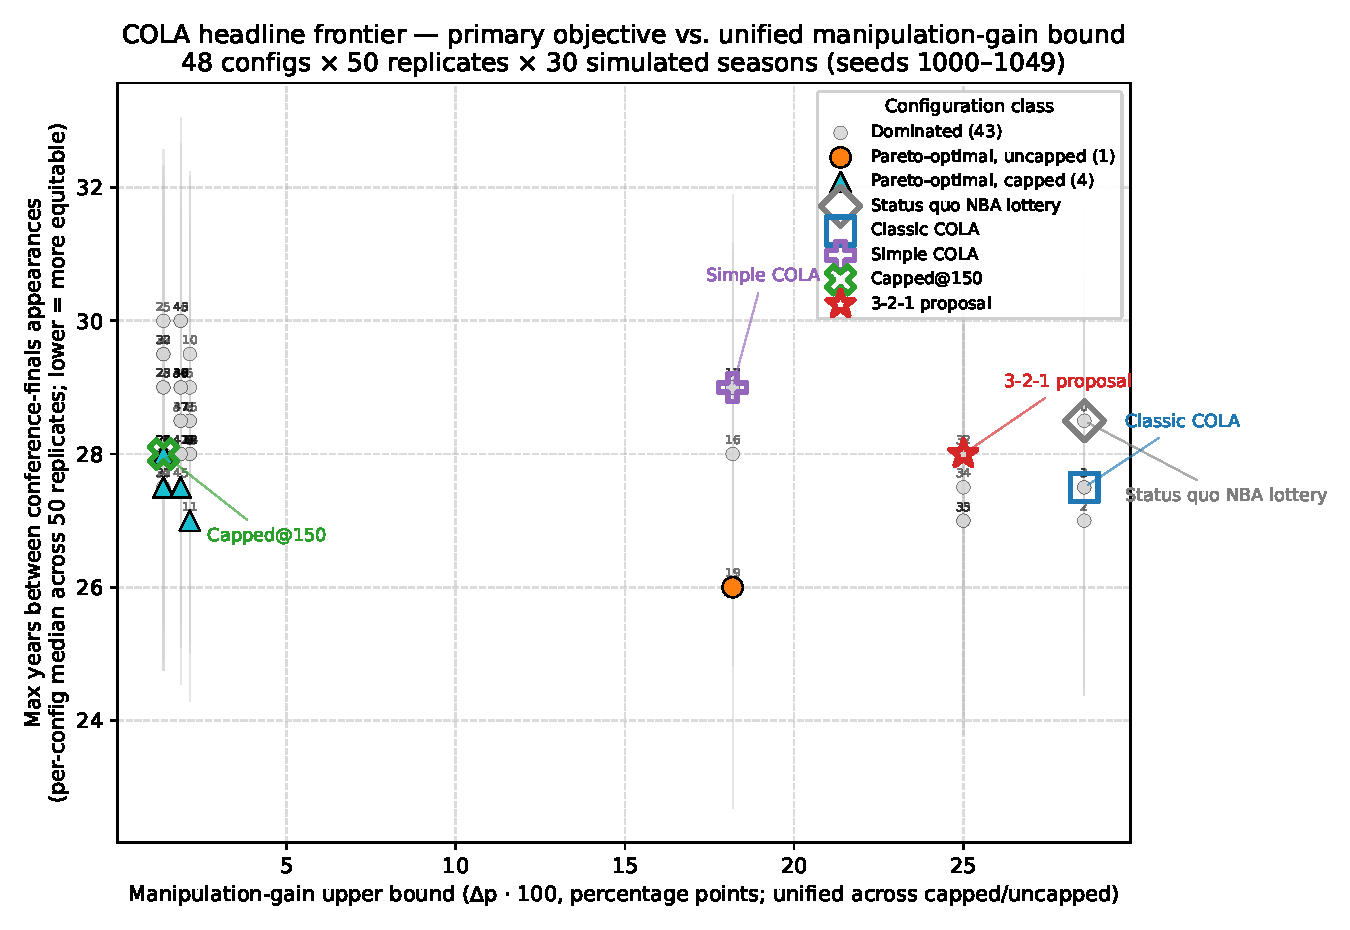
\includegraphics[width=0.85\linewidth]{figures/pareto_primary_vs_manipulation.pdf}
\caption{Headline Pareto frontier in the (max-yrs-CF, manipulation-gain) plane. Y-axis: median maximum years between conference-finals appearances across $50$ replicates (lower is better). X-axis: closed-form manipulation gain $\Delta p$ as a percentage (lower is better). The X-axis spans two analytical regimes: uncapped configurations sit at $\Delta p \approx 4 / |E|$ (Classic / Simple / Status quo / 3-2-1); capped configurations collapse to $\Delta p \approx 0.3 / |E|$ (Corollary~\ref{cor:cap-cancels}), creating the tight band at the left. The third dominance dimension (rank-1-to-5 spread) is not visualized; see Table~\ref{tab:pareto-set} for the full universal-dominance set.}
\label{fig:pareto-manip}
\end{figure}

The headline finding is operational. Under the three-dimensional universal-dominance comparison the framework supports, the cross-variant choice the league faced in the 2026 design discussion collapses to a single Pareto-relevant named variant. The other three \cola{} variants and the 2026 3-2-1 proposal are not on the frontier under any choice of league weighting over the three dominance objectives. The Pareto frontier itself is not a singleton: four unnamed configurations (cids 11, 19, 31, 45) trade max-yrs-CF for manipulation gain or rank-spread, sweeping a strip in the dial space worth further exploration in §\ref{sec:discussion}.

\subsection{Cap-Cancels-Out: Empirical Confirmation}
\label{sec:sweep-cap-cancels}

Corollary~\ref{cor:cap-cancels} establishes analytically that the cap value $C$ drops out of the Capped configuration's manipulation-gain bound: $\Delta p_{\text{capped}} \leq \kappa / |E|$. The sweep confirms the cancellation directly. The grid contains $36$ capped configurations: three pool settings ($|E| = 14, 22, 16$-tiered), three cap values ($C \in \{100, 150, 200\}$), and four scopes.
\begin{itemize}
    \item All $12$ capped configurations at $|E| = 22$ realize $\Delta p = 1.364\%$ (median across $50$ replicates, std $0$); closed form $\kappa / |E| = 0.3 / 22 \approx 1.364\%$.
    \item All $12$ capped configurations at $|E| = 14$ realize $\Delta p = 2.143\%$ ($0.3 / 14 \approx 2.143\%$).
    \item All $12$ capped configurations at $|E| = 16$ (tiered) realize $\Delta p = 1.875\%$ ($0.3 / 16 = 1.875\%$).
\end{itemize}
The realized manipulation gain is invariant across $C \in \{100, 150, 200\}$ within each eligibility setting. The capped configurations on the Pareto frontier (cid 11 at $|E| = 14$, cids 26 and 31 at $|E| = 22$, cid 45 at 16-tiered) and the capped configurations off the frontier exhibit the same per-$|E|$ value of $\Delta p$.

The policy implication is operational. A league considering a Capped configuration can choose $C$ on the basis of per-team accumulation speed and per-series tanking cost (Lemma~\ref{lem:capped-bound} ties the per-series cost to $0.3 \cdot C$) without changing the manipulation-gain ceiling, which is fixed by $|E|$. To lower the manipulation-gain ceiling, the lever is the eligibility pool, not the cap.

\subsection{Reset-on-Championship as a Winning Scope}
\label{sec:reset-on-championship}

Three of the five Pareto-optimal configurations (cids 11, 19, 31) use the reset-on-championship carry-over scope. One uses bounded-30yr (cid 26, the Capped@150 named variant) and one uses unbounded (cid 45). The single-season scope does not appear on the Pareto frontier at all; the 3-2-1 proposal (cid 32) is dominated, and no other single-season configuration in the grid clears.

The mechanism behind this finding is straightforward. Reset-on-championship is event-based: the league champion's identity is observable at one point each season, and the reset triggers across the entire pool at that one point. The scope retains the multi-year accumulation that distinguishes the \cola{} family from single-season mechanisms, while preventing index inflation that single-team unbounded accumulation would otherwise produce. Bounded-30yr (cid 26) is the cap-driven analog; unbounded (cid 45) appears on the frontier only when paired with the 16-tiered pool, which structurally limits the maximum accumulation per team via the tiering. We defer deeper interpretation of why this event-based scope dominates time-bounded scopes (bounded-30yr, unbounded) to Section~\ref{sec:discussion}.

\subsection{Historical Backtest}
\label{sec:backtest}

The backtest computes \cola{} state for every team across 26 NBA seasons (1999--2025) using verified Basketball Reference data: 775 team-season records, 776 first-round draft picks, and 55 lottery-day-attributed pre-draft pick trades. The engine separates pre-draft state (Phase A, used for draft-probability calculations) from post-draft diminishment (Phase B, carried forward to the next season). Cold-start effects stabilize by approximately season 5; we report aggregates over 21 stable seasons (2005--2025). The backtest is \emph{static}: it applies \cola{} rules to actual historical outcomes. Under a real \cola{} regime, draft outcomes would differ in ways that change future drought lengths and indices. We caveat the comparative cross-variant claims accordingly. An audit of all 364 lottery picks (14 picks $\times$ 26 seasons) identified $8$ instances where the draft-day holder differed from the lottery-day holder via post-lottery trades; \cola{} uses \emph{lottery-day} attribution.

The 2013--14 through 2016--17 Philadelphia 76ers are the canonical strategic-tanking sequence in modern NBA history: four consecutive top-3 lottery outcomes (picks \#3, \#3, \#1, \#3) acquired through deliberate multi-season non-competitiveness. Under the current weighted lottery, each tanked season yielded a top-tier pick. Under Classic \cola{}, graduated diminishment makes the same sequence self-defeating. Philadelphia's Classic \cola{} trajectory: $2{,}750$ in 2013--14 (rank 8/14) $\rightarrow$ $2{,}375$ in 2014--15 (9/14) $\rightarrow$ $2{,}188$ in 2015--16 (10/14) $\rightarrow$ $1{,}000$ in 2016--17 (14/14). Each top-3 pick triggers graduated diminishment ($\#1$: full reset; $\#3$: 50\% reduction), leaving Philadelphia at the bottom of the lottery pool by the fourth tanking season despite a 10--72 record. The Sacramento Kings hold the top Classic \cola{} index throughout this period, climbing from $7{,}250$ in 2013--14 to $10{,}250$ in 2016--17 via organic non-competitiveness. The Classic diminishment schedule ($\{1.0, 0.75, 0.5, 0.25\}$ for picks \#1--4) dominates the $\alpha = 1{,}000$ annual accumulation; a team that receives a top-3 pick in year $t$ cannot re-enter the top of the lottery in year $t + 1$ through tanking alone.

The Capped \cola{} cap calibration sweep over $\Max \in \{75, 100, 125, 150, 175, 200\}$ across the 21 stable seasons replicates the published default of $\Max = 150$ \citep{highley2026solvable5}: at $\Max = 150$, a mean of $1.62$ teams sit at the cap (range 0--3), matching the design target of fewer than two teams at the maximum on average. Sub-100 caps over-compress the rank-1-vs-rank-5 separation; caps above 175 erase the cap's purpose by leaving fewer than one team at the cap on average. This backtest is a second-tier validation alongside the headline Pareto result of Section~\ref{sec:pareto-frontier}: the static historical data confirms the qualitative comparative-statics the simulated sweep reports under closed-loop dynamics. We flag trade handling as a practical implementation question for any \cola{} deployment, following \citet{highley2026solvable4}'s recommendation of original-holder diminishment paired with a strengthened Stepien Rule.

\subsection{Sensitivity and Stability}
\label{sec:sensitivity}

A sensitivity pass on the Pareto-optimal set and the five named variants (a deduplicated subset of $9$ configurations) evaluates the headline at $N = 30$ and $N = 100$ replicates. The mean of the primary objective (max-yrs-CF) does not shift by more than $10\%$ from $N = 30$ to $N = 100$ on any subset configuration. The headline $N = 50$ is statistically sufficient for the dominance ordering reported in Section~\ref{sec:pareto-frontier}. Within-subset Pareto recomputation at $N = 30$ and $N = 100$ produces small membership flips ($N = 30$ Pareto subset $= \{0, 11, 19, 26, 45\}$; $N = 100$ Pareto subset $= \{31\}$), but these reflect within-subset re-ordering, not full-grid instability; the headline $N = 50$ Pareto set $\{11, 19, 26, 31, 45\}$ is the canonical answer. The closed-form manipulation-gain dimension is invariant across $N$ by construction.

\section{Discussion and Open Directions}
\label{sec:discussion}

The bounds in this paper formalize the manipulation-resistance properties of the \cola{} family. Theorem~\ref{thm:bound} bounds the open assumption (4) in Classic \cola{}'s incentive-compatibility argument at approximately $4\%$ under empirically calibrated parameters, with explicit sensitivity to $T_{\max}$, $T_{\text{boundary}}$, $n$, and $\bar{k}$. Lemma~\ref{lem:capped-bound} bounds the per-series exposure that Capped \cola{}'s stockpile cap was designed to address. Combined, the four manipulation channels available under Capped \cola{} (single-season tanking, pool manipulation, multi-year strategic tanking, and per-series playoff tanking) compose to a small joint exposure relative to the status-quo lottery, where repeat tanking has memoryless returns.

\subsection{3-2-1 as 2026 Stopgap, \cola{} as 2029 Candidate}

The NBA's 2026 ``3-2-1'' proposal \citep{highley2026threetwoone} is structurally a uniform lottery with an adjustment for the play-in tournament and a reduction for the three teams at the bottom of the standings. The proposal includes a three-year re-evaluation provision; the design discussion is expected to reopen in 2029. We read 3-2-1 as a short-horizon stopgap that accepts the Munro-Banchio tradeoff (uniform-style flattening, with the worst teams given fewer balls than the middle of the lottery pool). \cola{} is the natural candidate for the 2029 re-evaluation on a different design axis: dial $S$ (carry-over scope) shifts the priority basis from single-season records to multi-year playoff history, an option neither 3-2-1 nor any single-season mechanism considers.

The choice between 3-2-1 and \cola{} is the choice between two answers to the Munro-Banchio impossibility. 3-2-1 sacrifices differential reward for non-tanking. \cola{} preserves differential reward across years by relocating it to a non-manipulable basis. The 2029 discussion will benefit from having both options analytically characterized.

\subsection{Dial-Space Adoption Tradeoffs}

Each dial of Section~\ref{sec:family} matters more to some audiences than others. Three audience groups frame the adoption tradeoffs differently.

\emph{Fans and media} care most about $E$ (eligibility) and $W$ (lottery weighting). The current 14-team weighted lottery fits a 30-second broadcast graphic; Capped's exclusion-rule pool and Countdown's nested Monte Carlo do not. Variants that simplify the eligibility rule (Simple, Classic) are easiest at this layer.

\emph{General managers and owners} care most about $\Delta$ (increment) and $\rho$ (diminishment). A multi-year rebuild requires a forecastable trajectory: Classic's flat $\Delta = \alpha$ and graduated $\rho$ are the most tractable. Capped's wins-based $\Delta$ and six-step $\rho$ add complexity but remain forecastable. Countdown's $\Delta = d \cdot w$ multiplies two factors that move in opposite directions for a rebuilding team and produces noisier multi-year forecasts.

\emph{League counsel} cares most about $S$ (carry-over scope). Multi-year scopes introduce questions that single-season scopes (3-2-1, the legacy lottery) avoid: how does mid-season team relocation, ownership change, or league realignment interact with carry-over priority? Reporting requirements and ambiguity both grow with $S$. The NBA's apparent preference for single-season-scope mechanisms in 3-2-1 is consistent with $S$ being the dial under the most external pressure.

\newpage

\paragraph{Open directions:} three follow-on questions extend this work.
\begin{itemize}
    \item \emph{Tighter manipulation bound:} the structural anti-correlation in Definition~\ref{def:anticorr} is a calibrated assumption rather than a formally derived consequence of the mechanism. A stationarity argument that bounds $T_{\text{boundary}}$ as a function of league parameters (number of teams, season length, playoff structure) would close assumption (4) entirely.
    \item \emph{Pick-value gap:} combining the probability bound (this paper) with a separate bound on the pick-value gap $d_k - d_{k+1}$, derived from the distribution of draft-eligible prospect quality, would close the manipulation incentive in absolute terms, not just in probability.
    \item \emph{Axiomatic embedding:} the lift from \citet{coreno2022axiomatic}'s axioms (RP, EF1, SP) to multi-period priority mechanisms remains open. Section~\ref{sec:fairdiv} flags the question; a formal verification would embed \cola{} in the assignment-mechanism literature and clarify which one-period impossibilities transfer to multi-period settings.
\end{itemize}

A reproducibility artifact accompanies this paper: an interactive backtester implementing all five \cola{} variants plus the 3-2-1 proposal across 26 NBA seasons, with locked-seed Monte Carlo for Countdown \cola{} probabilities \citep{rajan2026explorer}.

\bibliographystyle{unsrtnat}
\bibliography{references}

\end{document}
